\section{Mail headers analysis}


\subsection{Mail headers dump}


\subsubsection{Identity and organization of the sender}

The two mail were sent by Marta (using the address \email{marta@salleurl.edu}) and Rick (using the address \email{rick@salleurl.edu}), respectively. The organization to which they belong to is the \emph{La Salle Ramon Llull University} as can be inferred from the domain of their email addressese: \texttt{salleurl.edu}.

In the case of Rick, the \texttt{X-Authentication-Warning} header suggests that the content of the \texttt{From} header could have been forged (but probably wasn't, for the reasons described at the following URL: \url{http://www.slingcode.com/pineauthenticationwarning.php}).


\subsubsection{Mail clients used to send the messages}

Marta is probably using Microsoft Outlook Express, version 6.00.2800.1158 to send their emails as shwon in the \texttt{X-Mailer} header. In Rick's case, no \texttt{X-Mailer} header is provided, but the combination of the information provided by the \texttt{X-Authentication-Warning} and \texttt{Message-ID} headers almost certainly indicate that the mail was sent using Pine\footnote{Pine is a tool for reading, sending and managing emails, developed by UW Technology at the University of Washington: \url{http://www.washington.edu/pine/}.}.

It is worth to note that the headers which were used to retrieve this information can easily be forged by the message sender and they could thus report incorrect data.


\subsubsection{Network addresses}

The different network addresses extracted from the email headers are: \texttt{10.0.14.198}, \texttt{130.206.42.238} and \texttt{130.206.42.246} for the email sent by Marta to Pete and \texttt{127.0.0.1} (the not that useful loopback address), \texttt{130.206.42.238} and \texttt{130.206.42.246} for the email from Rick to Pete.

A communication diagram for the two email which also includes the IP addresses of the involved parties, is represented in the Figure~\vref{fig:mail}.


\subsubsection{Network software and versions}

The network softwares used by the involved parties are \texttt{sendmail} (used by the LaSalle University network) and \texttt{qmail} (used by Pete's email provider).

It is possible to retrieve \texttt{sendmail}'s version by analyzing the headers: \texttt{columba.salleurl.edu} is running version {\tt 8.12.9} while \texttt{relay1.salleurl.edu} is running version {\tt 8.12.8p1}. Additionally, in the second email transaction, \texttt{sendmail} also exposes the underlying operating system for \texttt{columba.salleurl.edu}: \texttt{Debian 3}.

As already seen in the preceding answer, network software and versions are also included in the communication diagram \vpageref{fig:mail}.


\subsubsection{Domains}

As done with the IP addresses, domains can also easily be extracted from the email headers. The already cited {\tt columba.salleurl.edu} and {\tt relay1.salleurl.edu}; the originating server for the first email: {\tt LEGOLAS}; and Pete's email provider: {\tt fithwor.pair.com} were found. The two email domains {\tt salleurl.edu} and {\tt isecom.org} can also be listed here.

Together with the IP addresses and the newtork softwares, domains are also shown in the Figure~\vref{fig:mail}.

\begin{figure}[p]
	\centering

	\subfloat[fig:marta-pete][Email from marta to pete]{
		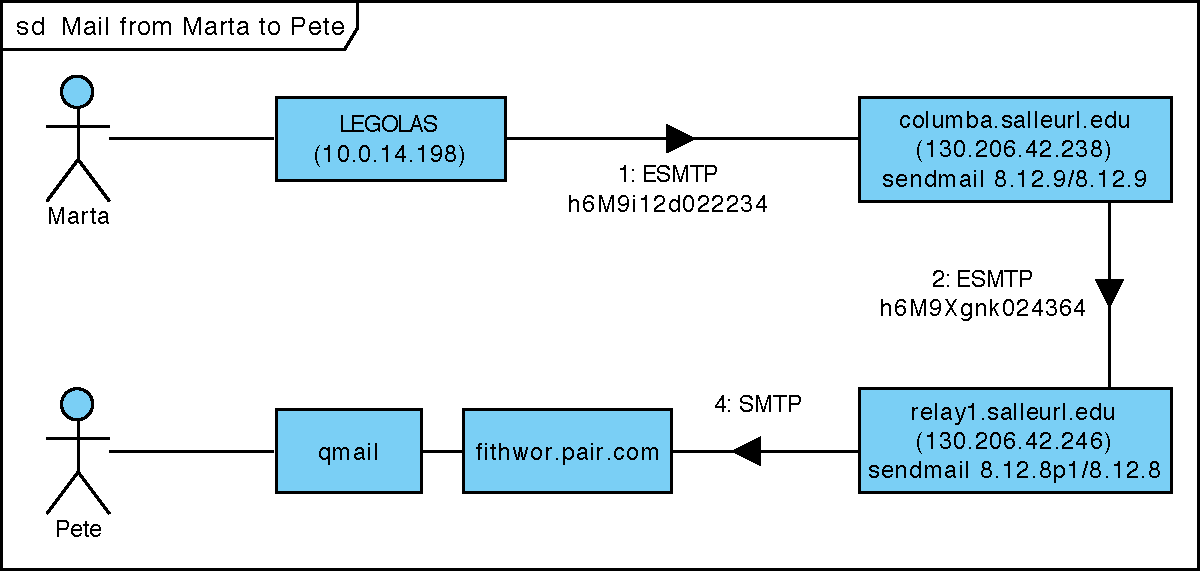
\includegraphics[scale=0.5]{uml/marta-pete}
	}
	\\[10mm]

	\subfloat[fig:rick-pete][Email from Rick to Pete]{
		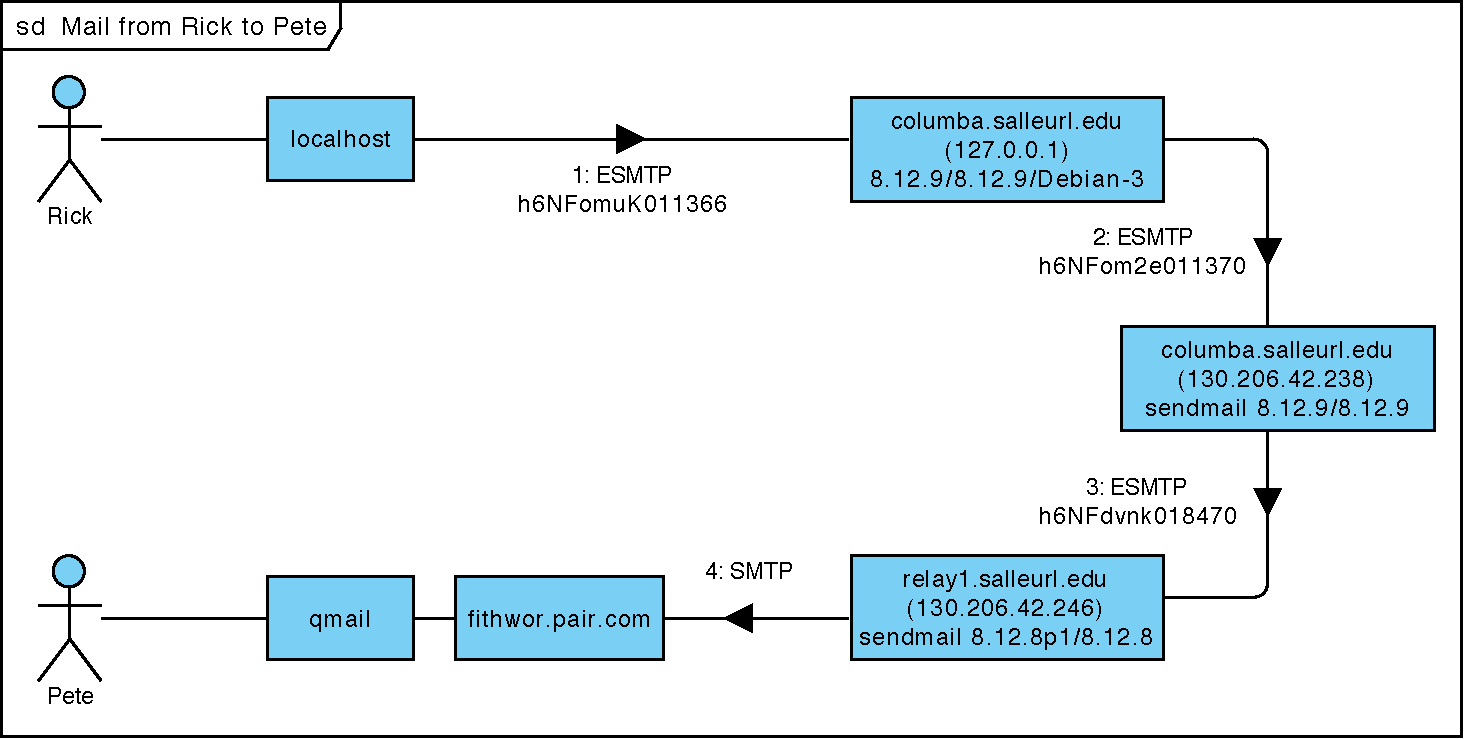
\includegraphics[scale=0.5]{uml/rick-pete}
	}
	\\[5mm]

	\caption{Communication diagrams for the different hosts intervening in the mail transmission between the three actors.}
	\label{fig:mail}
\end{figure}
